\documentclass[a4paper]{article}
%\usepackage{polski}
\usepackage[utf8]{inputenc}
\usepackage[T1]{fontenc}
\usepackage{graphicx}
\usepackage{multirow}
\usepackage{fancyhdr}
\usepackage{hyperref}
\pagestyle{fancy}
\begin{document}
\begin{tabular}{p{7cm}r}
\textbf{Michał Radmacher}&\multirow{10}{*}{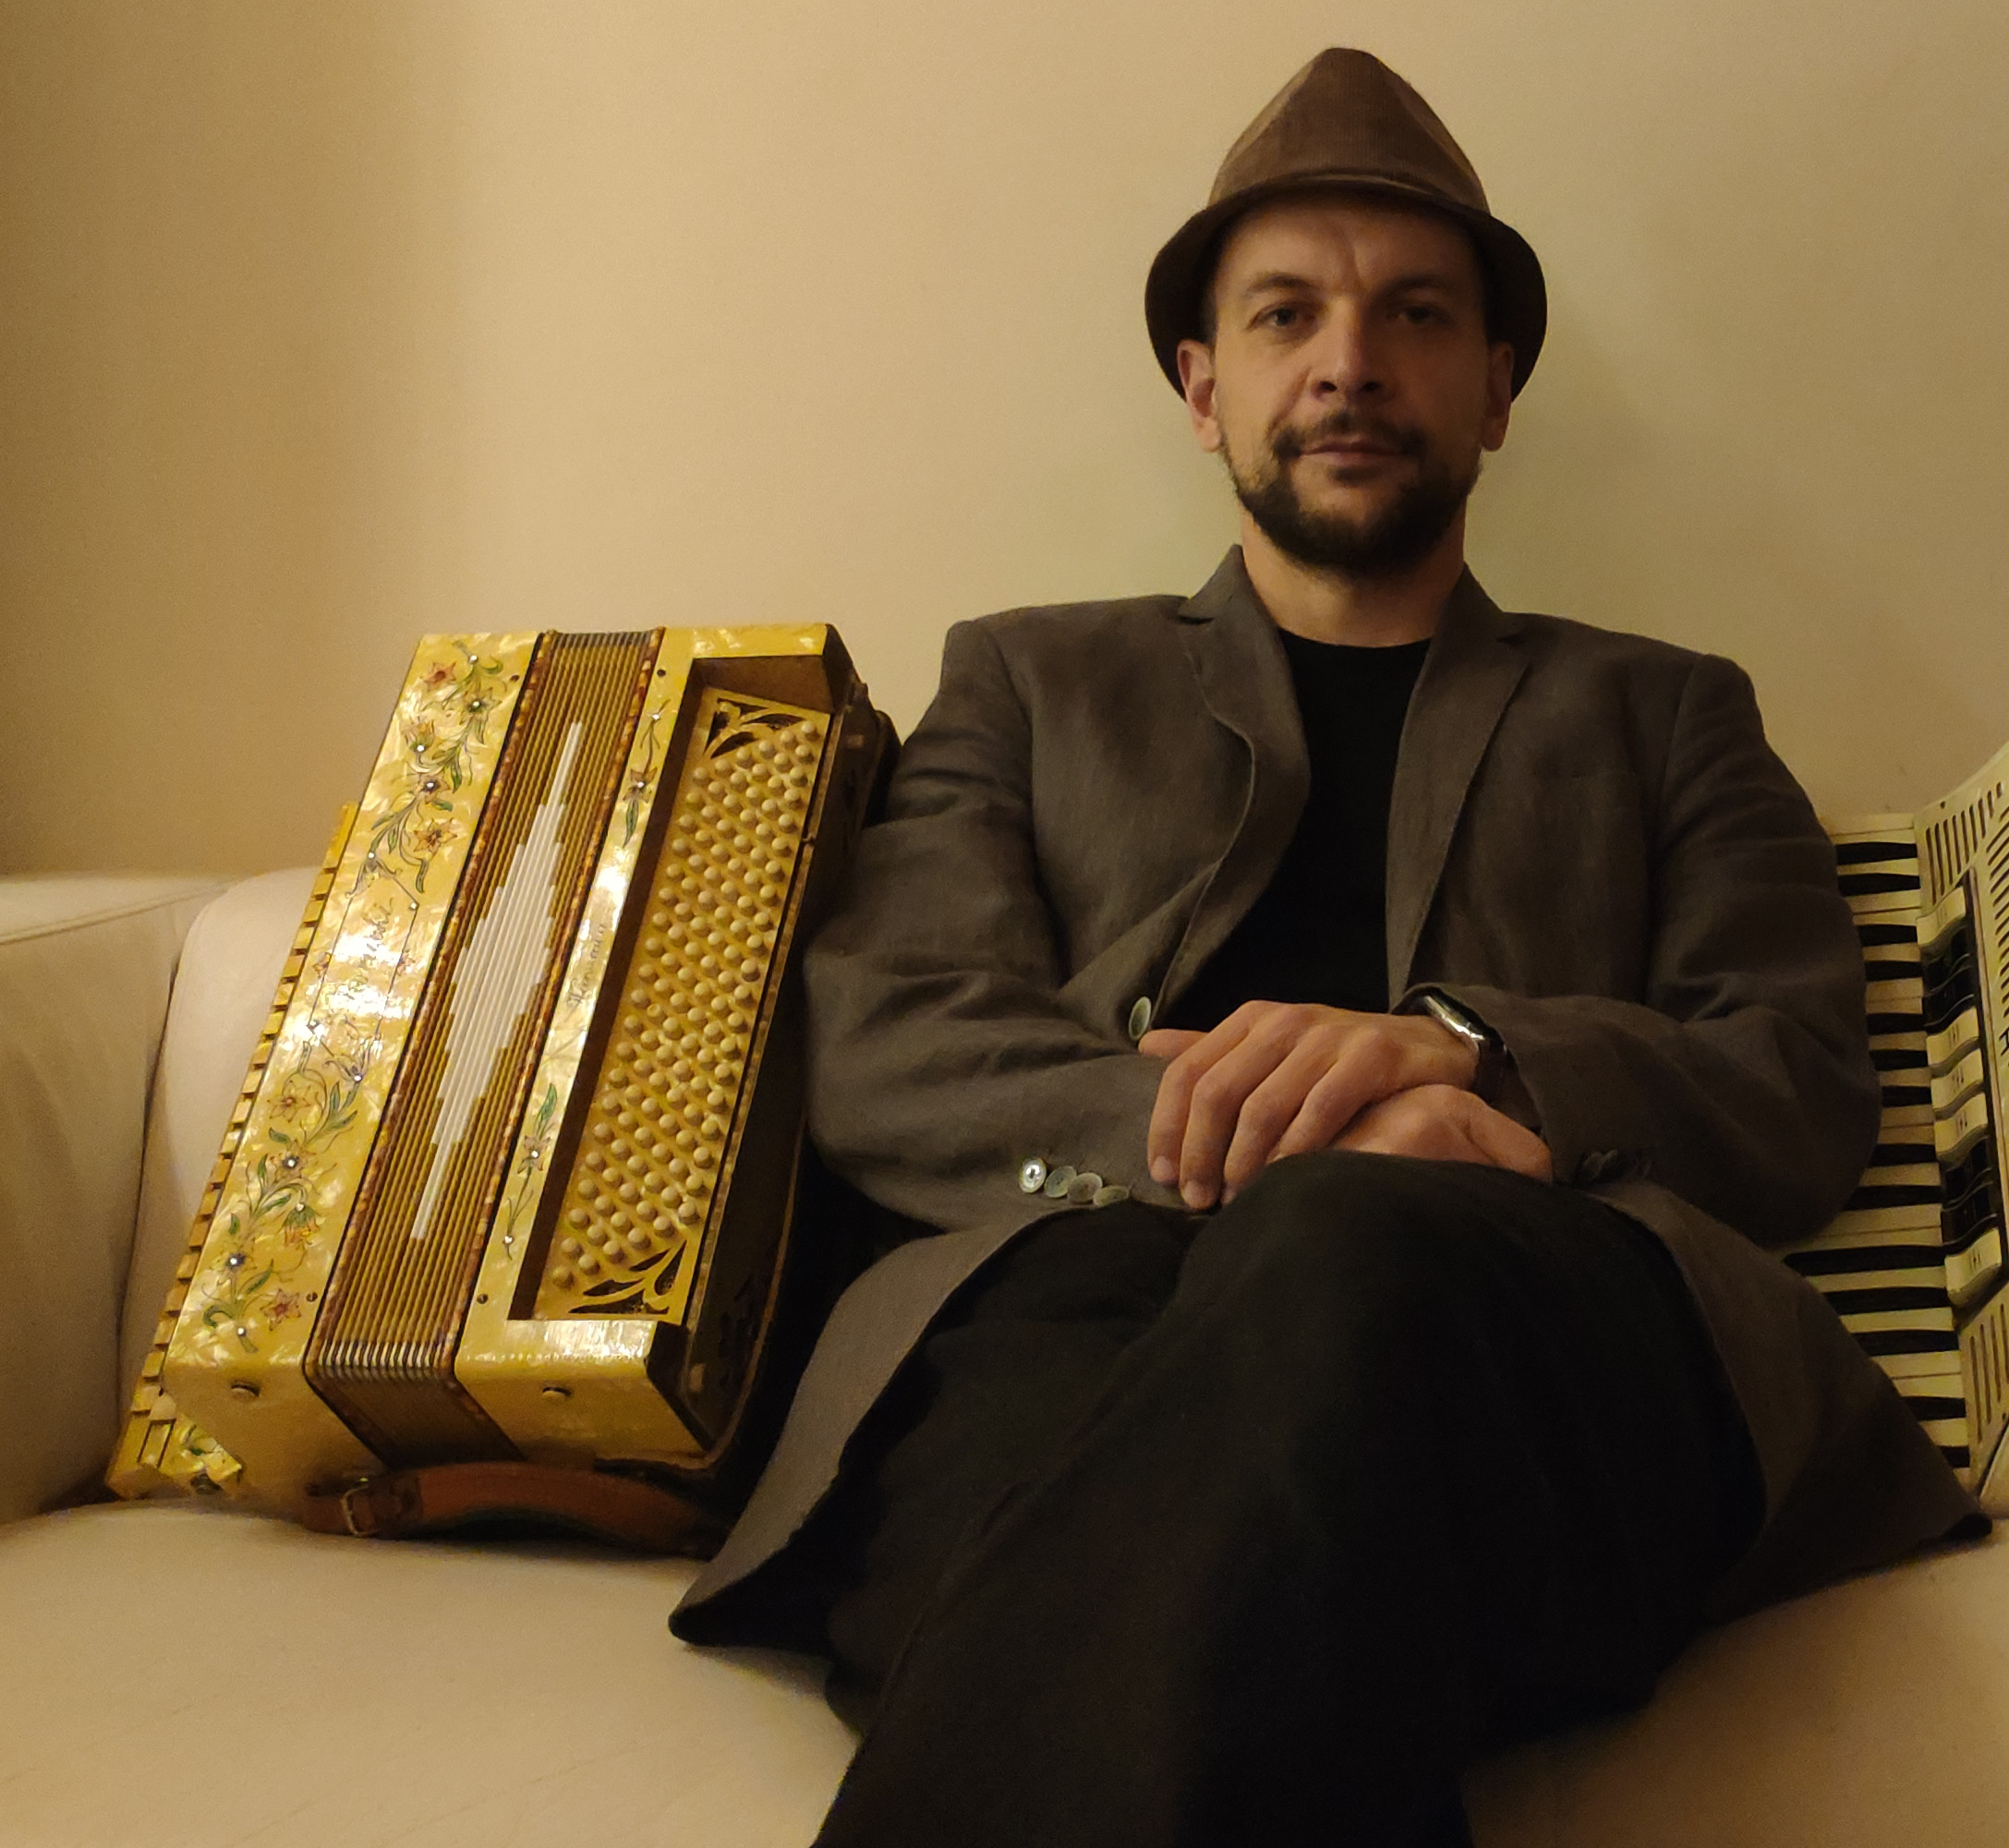
\includegraphics[width=40mm]{mr.jpg}}\\
&\\
+48 662 974 971&\\
michal@radmacher.pl&\\
\href{https://github.com/mradmacher/}{GitHub}\\
&\\
&\\
Lubię robić ciekawe projekty z ciekawymi ludźmi.
&\\
&
\end{tabular}

\subsection*{\center{Zawodowo}}

\begin{itemize}
  \item
  od 03.2014,
  CipherHealth
  \begin{itemize}
    \item
      branża medyczna; oprogramowanie wspierające edukację, zaangażowanie i satysfakcję pacjentów; rozwijanie kluczowych produktów, integracja z systemami zewnętrznymi, automatyzacja komunikacji z pacjentami
    \item
      \textbf{Ruby}, MongoDB, PostgreSQL, Cloud technologies
  \end{itemize}
  \item
    09.2012-02.2014,
    Polcode
    \begin{itemize}
      \item
        projektowanie i rozwój aplikacji webowych w bezpośredniej współpracy z międzynarodowymi klientami
      \item
        \textbf{Ruby on Rails}, PostgreSQL, JavaScript, HTML, CSS
    \end{itemize}
  \item
    02.2010-08.2012,
    Softelnet
    \begin{itemize}
      \item
        rozwój i utrzymanie systemu ewidencji dla jednego z wiodących operatorów telekomunikacyjnych w Polsce
      \item
        \textbf{PowerBuilder}, \textbf{PL/SQL}, SQL
    \end{itemize}
  \item
    11.2008-01.2010,
    Seihosoft
    \begin{itemize}
      \item
        projektowanie, rozwój i utrzymanie systemu wspierającego obsługę sieci sklepów
      \item
        \textbf{Java}, JMS, Hibernate
    \end{itemize}
  \item
    Open Source
    \begin{itemize}
      \item
        Stworzyłem aplikację dla geologów \href{https://github.com/mradmacher/paleolog}{PaleoLog}, która pomaga w gromadzeniu i analizie danych z prób mikropaleontologicznych
      \item
        Jestem muzykiem i zaprojektowałem strony dla swoich zespołów: \href{https://czarnymotyl.art}{https://czarnymotyl.art} \href{https://balkanartz.eu}{https://balkanartz.eu}, \href{https://karoryfer.com}{https://karoryfer.com}.
      \item
        Kilka gemów: \href{https://github.com/mradmacher/entitainer}{entitainer}, \href{https://github.com/mradmacher/param\_param}{param\_param}, \href{https://github.com/mradmacher/optiomist}{optiomist}
    \end{itemize}
\end{itemize}

\subsection*{\center{Naukowo}}
\begin{itemize}
  \item
    10.2005-05.2009 \textbf{inżynier}, Wyższa Szkoła Zarządzania i Bankowości w Krakowie, Informatyka

  \item
    10.2001-05.2005, Uniwersytet Jagielloński, Matematyka

  \item
    1998-2004, muzyk instrumentalista,
    Szkoła II Stopnia im. Władysława Żeleńskiego w Krakowie
\end{itemize}

\subsection*{\center{Językowo}}
\begin{itemize}
\item
  \textbf{polski} --- ojczysty
\item
  \textbf{angielski}, hiszpański, rosyjski, bułgarski --- komunikatywny
\end{itemize}

\subsection*{\center{Na co dzień}}
\begin{itemize}
\item
  \textbf{Ruby}, JavaScript
\item
  Go
\item
  PostgreSQL, MongoDB
\item
  Linux
\item
  GIT
\item
  Vim
\end{itemize}

\subsection*{\center{Prywatnie}}
\begin{itemize}
\item
  Gram na klarnecie, akordeonie i kilku innych instrumentach.
\item
  Uczę się języków, zarówno tych ludzkich jak i komputerowych.
\item
  Trenuję karate.
\end{itemize}
\end{document}
